\section{Conclusion}

Online communication has created a convenient and simple method for us to connect and transmit data over communication channels. Thus, transferring information over the Internet requires higher level of security when it comes to sensitive data. This could be achieved through the means of cryptosystems and cryptography. Primitives of symmetric-key cryptography lay the foundation of our report. Surveying its mechanisms, we have implemented a simple chat application in Python that encrypts messages before transferring them over the Internet. Substitution and transposition ciphers, alongside block and stream ciphers have been introduced in our project. The palette of reviewed ciphers stretches from simple to more complex ones: Caesar cipher, ROT13, One-time pad, Vigenere cipher, Enigma machine, Rivest Cipher 4, Data Encryption Standard (DES), 3DES, Advanced Encryption Standard (AES). Existing modes of operations (ECB, CBC, CFB, OFB, CTR) that can be applied to block and stream ciphers were also presented as they allow for larger data to be encrypted in order to guarantee its confidentiality. A client-server architecture was built thanks to a TCP transport layer protocol with same IP address and port number. Once a connection was established, communication flow of messages was tested. The client script contains the encryption functions of the chosen four algorithms (Caesar cipher, ROT13, DES, AES) in order to encrypt messages before sending them to the server over the Internet. The recipient, aka the server, on the other side, is responsible for decrypting the messages, hence it holds all decryption operations, in order to echo back to the client the deciphered messages. These encryption and decryption techniques depend upon the type of data and the channel through which the data is being communicated. Throughout the report, we have drawn a comparison analysis of the proposed mechanisms based on their basic features, advantages, drawbacks and applications. The performance analysis, at the end, takes into account the speed factor, i.e., the time it takes for each algorithm to encrypt and decrypt messages. The results showed equal performance by Caesar cipher and ROT13. DES outperformed AES. Even though AES took more processing time, it proved to be the most secure encryption algorithm due to the initialization vector and the better mode of operation, CBC. DES does not have an IV and is built alongside a weak and simple mode of operation ECB. Moreover, nowadays, DES is considered as a weak encryption standard. In 2012, a system was designed to crack any DES key in 26 hours \cite{crack.sh}. Nevertheless, it can still be used for applications where sensitive data is not required. AES replaced DES as it is more powerful and offers a great number of possible keys, $2^{256}$, which has no comparison. Even the number of atoms in the universe is smaller than AES keys (with a range from between $10^{78}$ to $10^{82}$ \cite{atoms}. We suppose, even if we had many supercomputers to each test the $2^{256}$ keys per second, the time to crack AES would still be much longer than the age of the universe (estimated at 13.82 billion years \cite{universe}). The report concludes that encryption algorithms attempt to thwart risks posed by untrusted networks, such as the Internet. In response to these risks, we deploy methods to encrypt messages before sending them over the Internet, so that outside access is prevented and content is preserved. In fine, sensitive data encryption should be on the radar of enterprises, governments, banks, retailers, institutions of higher learning and health organizations nowadays.


\newpage 
\section{Appendix}
A link to the GitHub repository of the project: \url{https://github.com/dmarinova1/BSP-S3-Encryption-algorithms}

\begin{figure}[h!]
  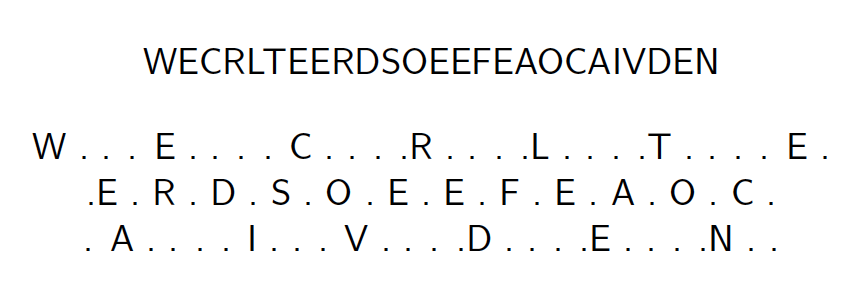
\includegraphics[width=\linewidth]{railfence.jpg}
  \caption{Rail Fence Cipher. Ref: Taken from Security I lecture notes}
  \label{fig:railfence}
\end{figure}

\begin{figure}[h!]
  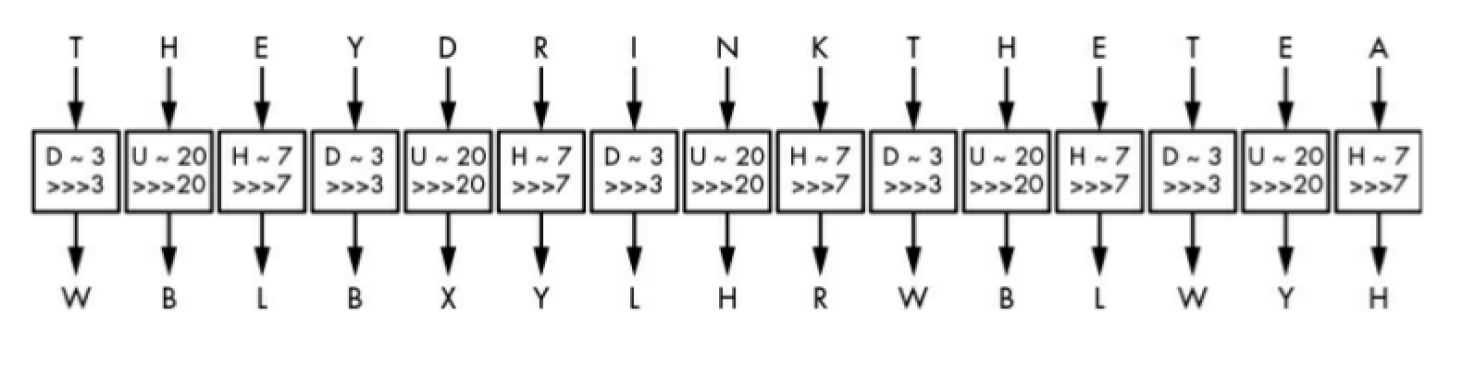
\includegraphics[width=\linewidth]{vigenere.jpg}
  \caption{Vigenere Cipher. Ref: Taken from Security I lecture notes}
  \label{fig:vigenere}
\end{figure}

\begin{figure}[h!]
  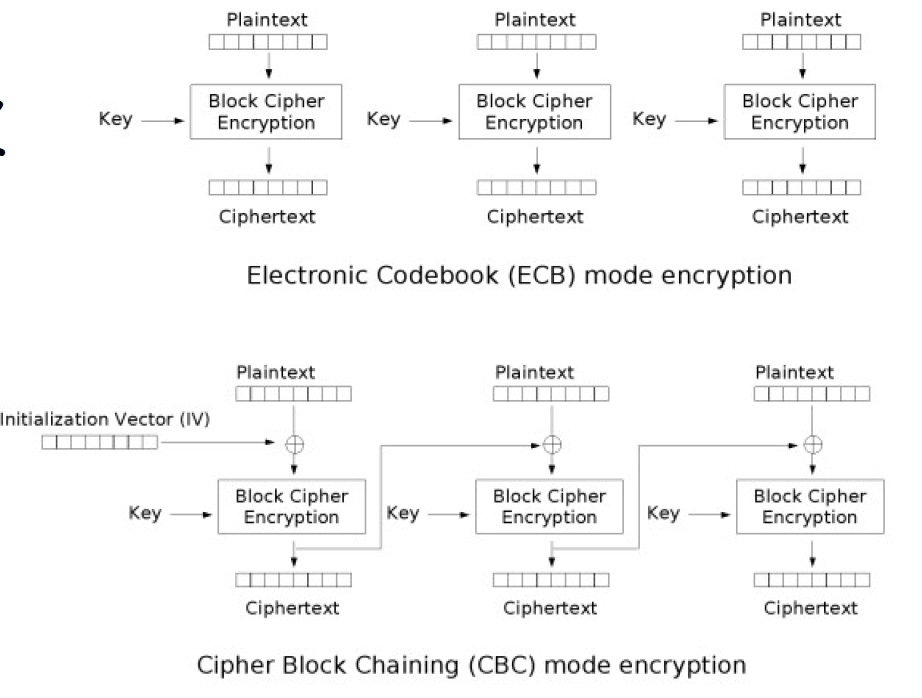
\includegraphics[width=\linewidth]{modes.jpg}
  \caption{ECB and CBC modes of operation. Ref: Taken from Security I lecture notes}
  \label{fig:modes}
\end{figure}

\begin{figure}[h!]
  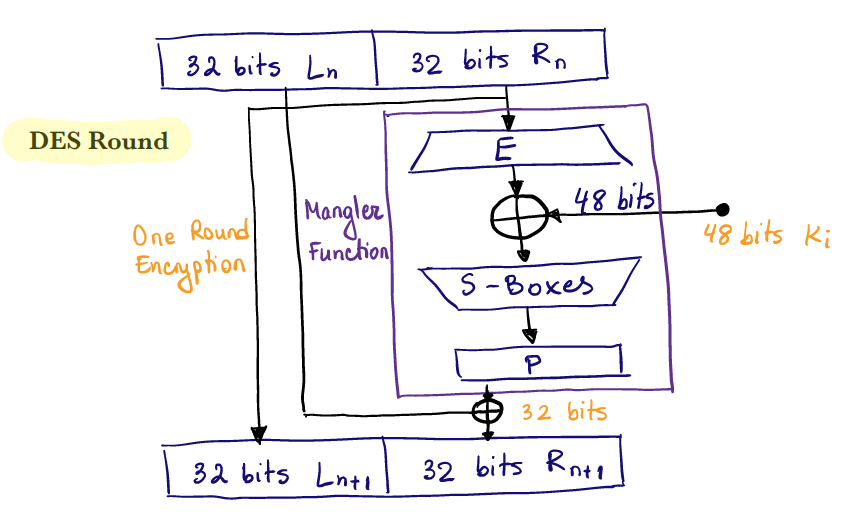
\includegraphics[width=\linewidth]{desround.jpg}
  \caption{DES Round Encryption. Ref: As presented in Security I course}
  \label{fig:desround}
\end{figure}

\begin{figure}[h!]
  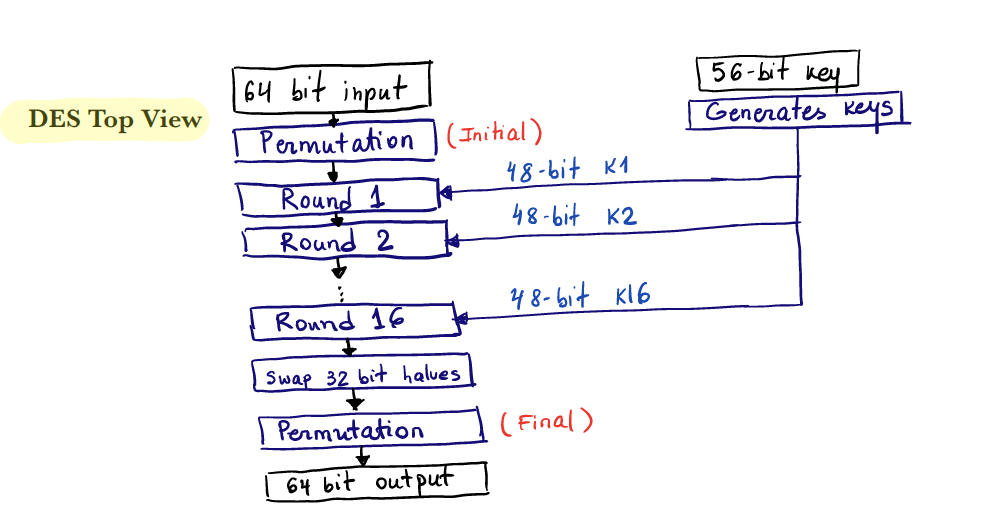
\includegraphics[width=\linewidth]{destopview.jpg}
  \caption{DES Top View. Ref: As presented in Security I course}
  \label{fig:destopview}
\end{figure}

\begin{figure}[h!]
  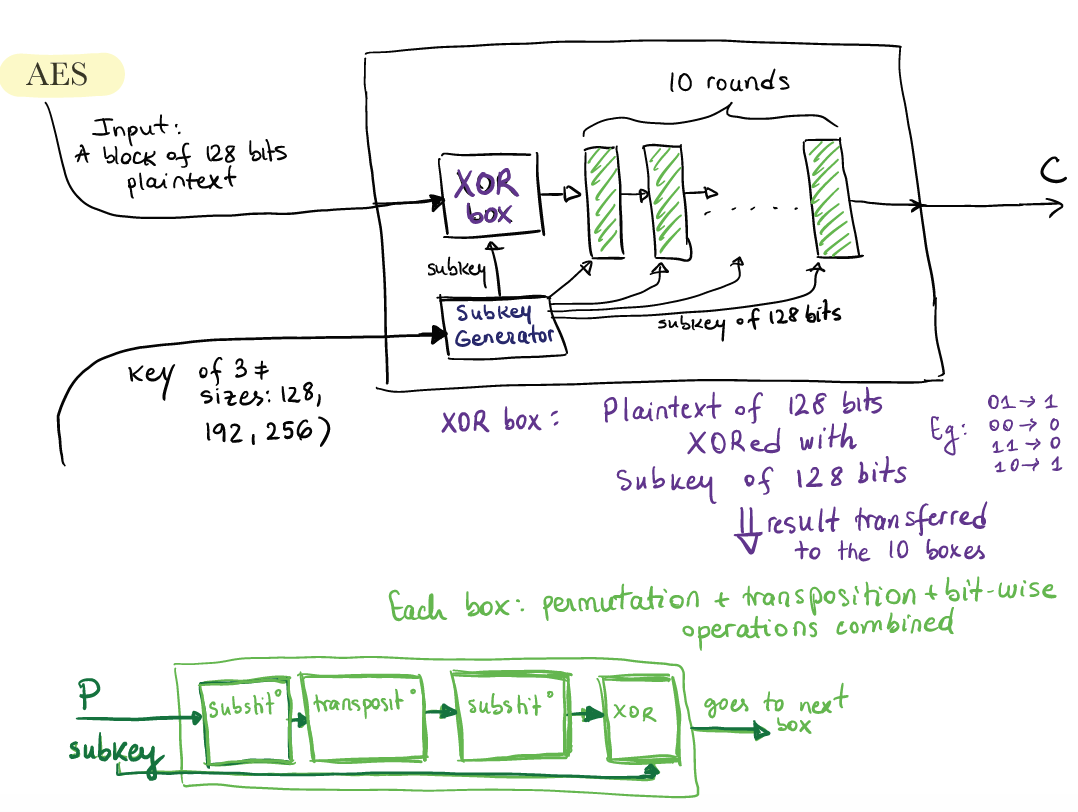
\includegraphics[width=\linewidth]{aes.jpg}
  \caption{AES. Ref: General idea from \textit{Cryptography and Network Security} by Stallings. Ed.7}
  \label{fig:aes}
\end{figure}
% that's all folks